\documentclass{report}
\usepackage{verbatim}
\usepackage{graphicx}
\title{DB3 REPORT}
\author{Ryan Wells -- 1002253W \n Chris James -- 1003019J}

\begin{document}
\maketitle
\newpage

%%%%%%%%%%%%%%%%%%%%%%%%%%%%%%%%%%%%%%%%%%%%%%%%%%%%%%%%%%%%%%%%%%%%%%%%%%%%
% Q1
%%%%%%%%%%%%%%%%%%%%%%%%%%%%%%%%%%%%%%%%%%%%%%%%%%%%%%%%%%%%%%%%%%%%%%%%%%%%
\section*{Query 1}
Query C is our optimized query. It has the lowest overall cost in
comparison to Query A and B and also a lower size cost. This is due to
Query A not having any nested queries and less projections than the
other two. \\
\subsection*{Query A}
\begin{verbatim}

/* Get a song that is on a bands album with the song 
   title occurs more than once and remove the duplicates
   (using HAVING count(*)>1) 
*/
SELECT BAND.NAME AS Band_Name, SONG.TITLE AS Song_Title
FROM BAND, SONG, RELEASE 
WHERE BAND.BID = RELEASE.BID AND SONG.RID = RELEASE.RID 
AND SONG.TITLE in
(
    SELECT TITLE
    FROM
    (
        Select TITLE, COUNT(TITLE)
        From Song 
        group by title
        having count(title)>1
    )
)
GROUP BY BAND.NAME, SONG.TITLE
HAVING count(*)>1
ORDER BY BAND.NAME
GO
\end{verbatim}
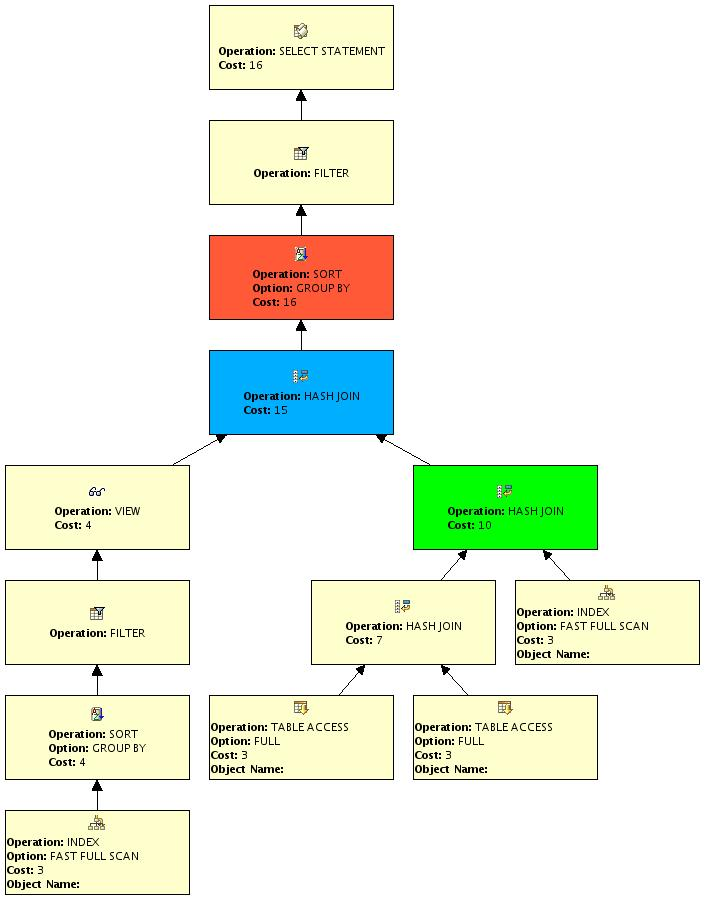
\includegraphics[width=0.8\textwidth]{Q1A}
\subsection*{Query B}
\begin{verbatim}
/*  Select songs where the titles match,
    the Songs Release ID's (RID) dont match,
    each song is on it's respective release,
    and the band has that song on one of its
    albums.    
*/
SELECT DISTINCT BAND.NAME AS Band_Name, S1.TITLE AS Song_Title
  FROM BAND,RELEASE R1,RELEASE R2 ,SONG S1, SONG S2
  WHERE S1.TITLE = S2.TITLE
  AND S1.RID <> S2.RID
  AND R1.RID = S1.RID
  AND R2.RID = S2.RID
  AND BAND.BID = R1.BID
  AND BAND.BID = R2.BID
ORDER BY Band_Name
\end{verbatim}
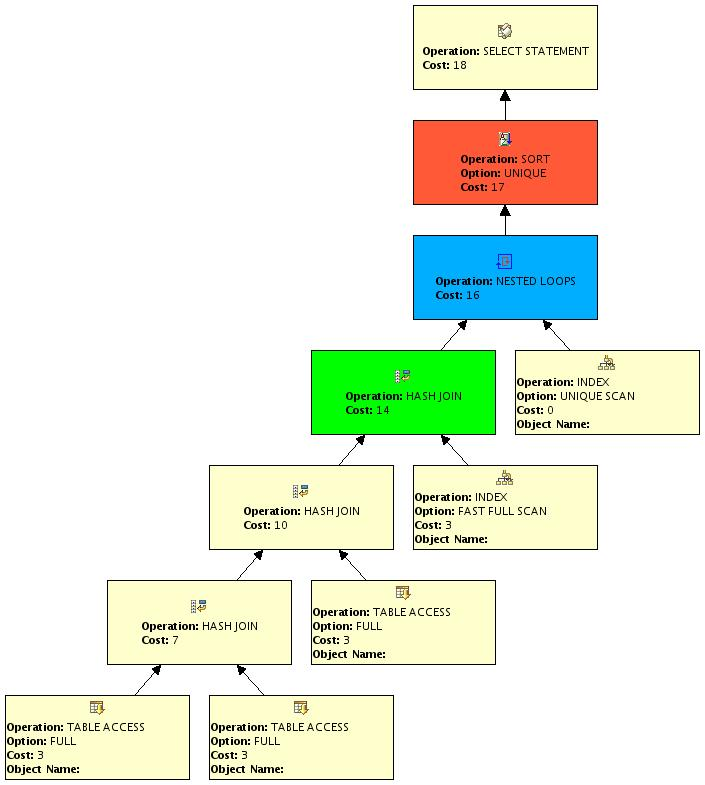
\includegraphics[width=0.7\textwidth]{Q1B}
\subsection*{Query C}
\begin{verbatim}
/*  Select every song that is on an album by a band
    and project only those that occur more than once
*/
SELECT BAND.NAME AS Band_Name, SONG.TITLE AS Song_Title
FROM BAND, SONG, RELEASE
WHERE BAND.BID=RELEASE.BID AND RELEASE.RID=SONG.RID
GROUP BY BAND.NAME, SONG.TITLE
HAVING count(*)>1
ORDER BY BAND.NAME
GO
\end{verbatim}
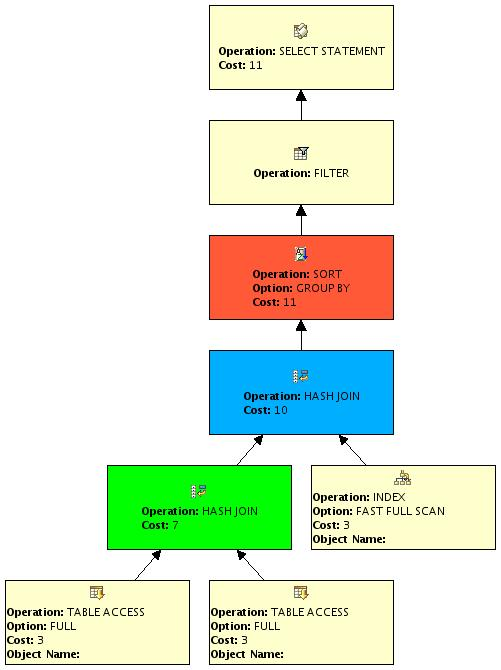
\includegraphics[width=0.7\textwidth]{Q1}
\subsection*{Output}
\begin{verbatim}
 BAND_NAME        SONG_TITLE                            
 ---------------  ------------------------------------- 
 Blind Guardian   Banish From Sanctuary                 
 Blind Guardian   Barbara Ann                           
 Blind Guardian   Goodbye My Friend                     
 Blind Guardian   Inquisition                           
 Blind Guardian   Journey Through The Dark              
 Blind Guardian   Lost In The Twilight Hall             
 Blind Guardian   The Quest For Tanelorn                
 Blind Guardian   Time What Is Time                     
 Blind Guardian   Traveler In Time                      
 Blind Guardian   Valhalla                              
 Blind Guardian   Welcome To Dying                      
 Bruce Dickinson  Accident Of Birth                     
 Bruce Dickinson  Book Of Thel                          
 Bruce Dickinson  Chemical Wedding                      
 Bruce Dickinson  Gates Of Urizen                       
 Bruce Dickinson  Killing Floor                         
 Bruce Dickinson  King In Crimson                       
 Bruce Dickinson  Laughing In The Hiding Bush           
 Bruce Dickinson  Tears Of The Dragon                   
 Bruce Dickinson  The Tower                             
 Bruce Dickinson  Trumpets Of Jericho                   
 Candlemass       A Sorcerer's Pledge                   
 Candlemass       At The Gallows End                    
 Candlemass       Bewitched                             
 Candlemass       Dark Are The Veils Of Death           
 Candlemass       Dark Reflections                      
 Candlemass       Demons Gate                           
 Candlemass       Mirror Mirror                         
 Candlemass       Samarithan                            
 Candlemass       Solitude                              
 Candlemass       The Well Of Souls                     
 Candlemass       Through The Infinitive Halls Of Death 
 Candlemass       Under The Oak                         
 Crimson Glory    In Dark Places                        
 Savatage         24 Hours Ago                          
 Savatage         Gutter Ballet                         
 Savatage         Hall Of The Mountain King             
 Savatage         Hounds                                
 Savatage         Legions                               
 Savatage         Of Rage And War                       
 Savatage         Sleep                                 
 Savatage         Strange Wings                         
 Savatage         When The Crowds Are Gone              

 43 record(s) selected
\end{verbatim}

%%%%%%%%%%%%%%%%%%%%%%%%%%%%%%%%%%%%%%%%%%%%%%%%%%%%%%%%%%%%%%%%%%%%%
% Q2
%%%%%%%%%%%%%%%%%%%%%%%%%%%%%%%%%%%%%%%%%%%%%%%%%%%%%%%%%%%%%%%%%%%%%
\section*{Query 2}
Query C is our optimized query. Even though A and B have the same
cost adding indices to either has reduced the cost. Also, we believe
that on a larger scale Query A should perform betteras the nested
query selecting only the songs that are a bonus song should reduce the
space complexity of the search. 
\subsection*{Query A}
\begin{verbatim}
/* First found all songs considered bonus sons (labelled BSONGS),
created a table of tuples featuring all bands with bonus songs.
Unioned this with a table of all band names and 0s marked as BONUSNUM.
Selected Max BONUSNUM values after Union*/
SELECT GPLAYERS.NAME AS Band_Name, MAX(BONUSNUM) AS Bonus_Num
FROM
(
    (
        SELECT BAND.NAME, Count(BSONGS.TITLE) AS BONUSNUM
        FROM BAND, RELEASE, 
        (
            SELECT *
            FROM SONG
            WHERE SONG.CDBONUS = 'Y'
        ) BSONGS
        WHERE BAND.BID = RELEASE.BID
        AND RELEASE.RID = BSONGS.RID
        GROUP BY BAND.NAME
        ) 
        UNION 
        ( 
            SELECT BAND.NAME, (0) AS BONUSNUM
            FROM BAND
        )
    ) GPLAYERS
GROUP BY GPLAYERS.NAME
\end{verbatim}
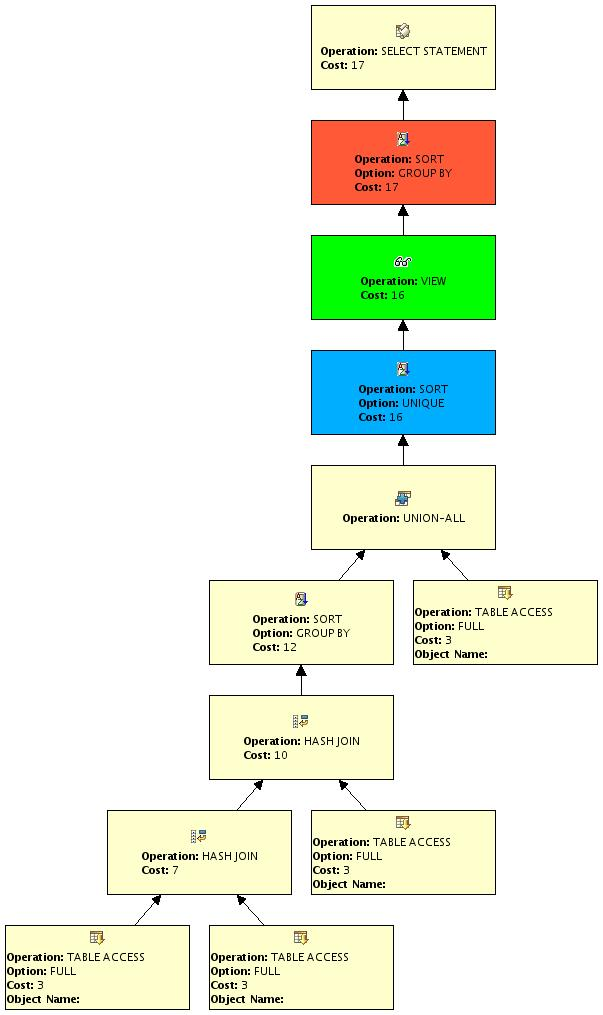
\includegraphics[width=0.7\textwidth]{Q2A}
\subsection*{Query B}
\begin{verbatim}
/*  Starting innermost, this is a union of (band name,0)
    tuples with (band name that has bonus tracks, number 
    of bonus tracks) as this will introduce the results
    of bands that have no bonus tracks. Taking the MAX
    of these will eliminate the duplicates (where elements
    with a bonus track occur twice due to this methodology)
    removes the duplicates (which will be the (band name,
    0) results).
*/
SELECT RESULTS.NAME AS Band_Name, MAX(RESULTS.TOTS) AS Bonus_Num
FROM(
    SELECT BAND.NAME,(0)as TOTS
    FROM BAND
    UNION
    SELECT BAND.NAME, COUNT(SONG.RID)
    FROM BAND, RELEASE, SONG
    WHERE BAND.BID=RELEASE.BID AND RELEASE.RID=SONG.RID AND
SONG.CDBONUS='Y'
    GROUP BY BAND.NAME
    )RESULTS
GROUP BY RESULTS.NAME
GO
\end{verbatim}
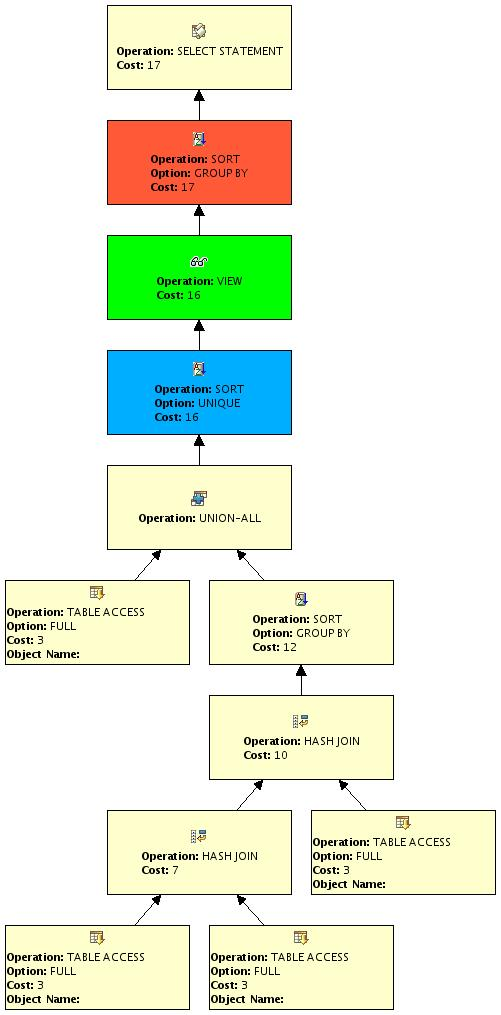
\includegraphics[width=0.7\textwidth]{Q2}
\subsection*{Query C}
\begin{verbatim}
/* First found all songs considered bonus sons (labelled BSONGS),
   created a table of tuples featuring all bands with bonus songs.
   Unioned this with a table of all band names and 0s marked as
   BONUSNUM.
   Selected Max BONUSNUM values after Union.

*/
CREATE INDEX bnames on BAND(NAME)
go
CREATE INDEX bsongs on SONG(CDBONUS)
go
SELECT GPLAYERS.NAME AS Band_Name, MAX(BONUSNUM) AS Bonus_Num
FROM
(
    (
        SELECT BAND.NAME, Count(BSONGS.TITLE) AS BONUSNUM
        FROM BAND, RELEASE, 
        (
            SELECT *
            FROM SONG
            WHERE SONG.CDBONUS = 'Y'
        ) BSONGS
        WHERE BAND.BID = RELEASE.BID
        AND RELEASE.RID = BSONGS.RID
        GROUP BY BAND.NAME
        ) 
        UNION 
        ( 
            SELECT BAND.NAME, (0) AS BONUSNUM
            FROM BAND
        )
    ) GPLAYERS
GROUP BY GPLAYERS.NAME
go
\end{verbatim}
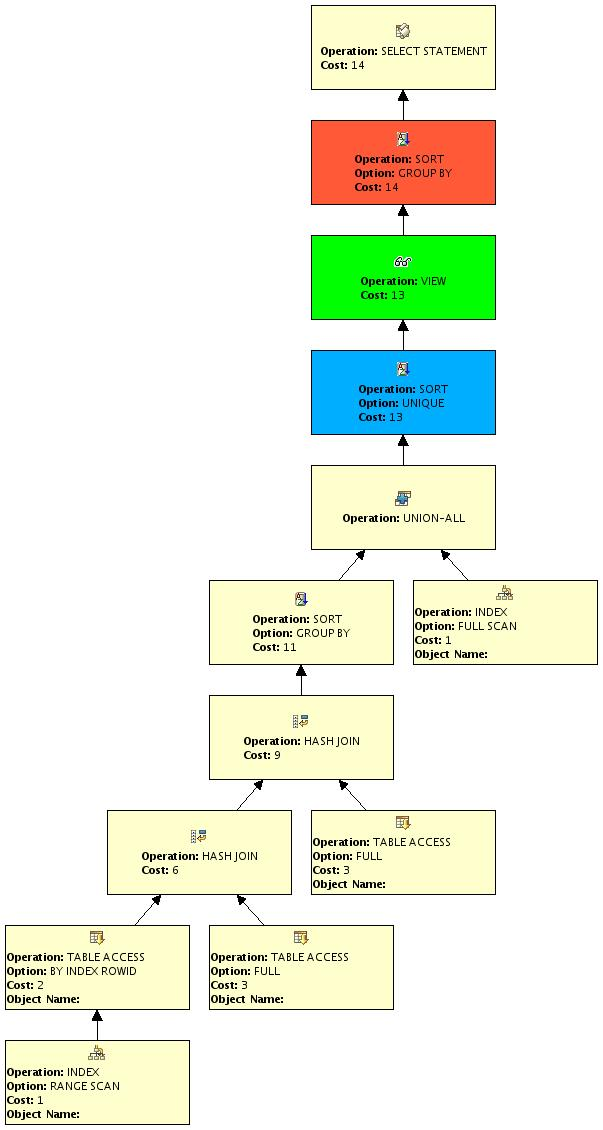
\includegraphics[width=0.7\textwidth]{Q2C}
\subsection*{Output}
\begin{verbatim}
 BAND_NAME           BONUS_NUM    
 ------------------  ------------ 
 Blind Guardian      6            
 Bruce Dickinson     0            
 Candlemass          1            
 Cirith Ungol        1            
 Crimson Glory       3            
 Dark Tranquility    0            
 Demons & Wizards    0            
 EverEve             1            
 Gamma Ray           1            
 Helloween           1            
 Iced Earth          1            
 Iron Maiden         0            
 Memento Mori        0            
 Nevermore           1            
 Opeth               2            
 Samael              0            
 Sanctuary           0            
 Savatage            6            
 Theatre Of Tragedy  0            
 Tristania           0            

 20 record(s) selected
\end{verbatim}

%%%%%%%%%%%%%%%%%%%%%%%%%%%%%%%%%%%%%%%%%%%%%%%%%%%%%%%%%%%%%%%%%%%%%%
% Q3
%%%%%%%%%%%%%%%%%%%%%%%%%%%%%%%%%%%%%%%%%%%%%%%%%%%%%%%%%%%%%%%%%%%%%%
\section*{Query 3}
Query C is our optimized query. We decided to optimize primarily by
using the faster ``UNION ALL'' instead of using ``UNION'' and having a
distinct higher up the table as this decreased the overall cost of the
query. Also adding two indices to the table has helped the overall
cost and the expense of making these indices was outweighed by this
gain. 
\subsection*{Query A}
\begin{verbatim}
/* Starting innermost, this unions the (BID,StartYear,EndYear) of a
   member where there is a start year relating to that members time in
   a band with the (BID,StartYear,EarliestRelease) where the
   EarliestRelease is the earliest release for that band member in
   that band and where the start year is null.
*/
SELECT MEMBER.NAME as Guitarist_Name, Band.Name as Band_Name,
Mems.STARTYEAR as Start_Year, MEMS.ENDYEAR as END_YEAR
FROM MEMBER, BAND,
(
    (
        SELECT BAND.BID,MEMBEROF.MID, MEMBEROF.STARTYEAR As STARTYEAR,
        MEMBEROF.ENDYEAR as ENDYEAR
        FROM MEMBEROF,BAND,RELEASE
        WHERE MEMBEROF.STARTYEAR>0 AND MEMBEROF.INSTRUMENT='guitar'
        AND MEMBEROF.BID=BAND.BID AND BAND.BID=RELEASE.BID
    )
    UNION
    (
        SELECT BAND.BID, MEMBEROF.MID, MIN(RELEASE.YEAR) AS year,
        MEMBEROF.ENDYEAR
        FROM BAND, RELEASE, MEMBEROF
        WHERE BAND.BID=RELEASE.BID AND MEMBEROF.INSTRUMENT='guitar' 
        AND MEMBEROF.BID = BAND.BID AND (MEMBEROF.STARTYEAR IS NULL)
        GROUP BY MEMBEROF.MID, BAND.BID,MEMBEROF.ENDYEAR
    )
) MEMS
WHERE MEMS.MID=MEMBER.MID AND BAND.BID=MEMS.BID
ORDER BY MEMBER.NAME, MEMS.STARTYEAR
go
\end{verbatim}
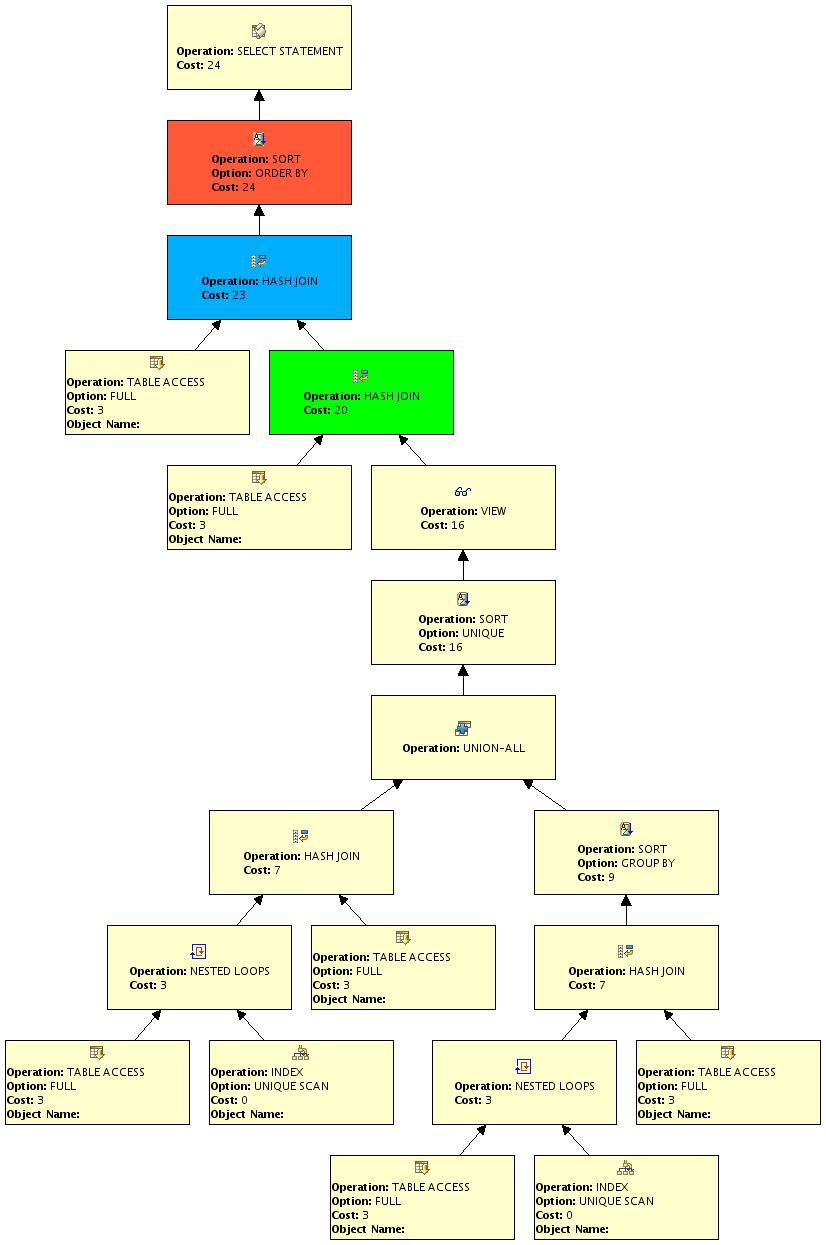
\includegraphics[width=0.7\textwidth]{Q3A}
\subsection*{Query B}
\begin{verbatim}
/* Starting innermost, this unions the (BID,StartYear,EndYear) of a
   member where there is a start year relating to that members time in
   a band with the (BID,StartYear,EarliestRelease) where the
   EarliestRelease is the earliest release for that band member in
   that band and where the start year is null.
*/
(
    SELECT MEMBER.NAME AS Guitarist_Name, BAND.NAME AS Band_Name,
    GPLAYERS.STARTYEAR AS Start_Year, GPLAYERS.ENDYEAR AS End_Year
    FROM MEMBER, BAND, 
    (
        SELECT * 
        FROM MEMBEROF 
        WHERE INSTRUMENT='guitar'
    ) GPLAYERS
    WHERE GPLAYERS.STARTYEAR IS NOT NULL
    AND GPLAYERS.MID = MEMBER.MID
    AND GPLAYERS.BID = BAND.BID
) 
UNION
(
    SELECT MEMBER.NAME AS Guitarist_Name, BAND.NAME AS Band_Name,
    FIRSTRELEASE.YEAR AS Start_Year, GPLAYERS.ENDYEAR AS End_Year
    FROM MEMBER, BAND, 
    (
        SELECT * 
        FROM MEMBEROF 
        WHERE INSTRUMENT='guitar'
    ) GPLAYERS, 
    (
        SELECT BID, MIN(RELEASE.YEAR) AS YEAR
        FROM RELEASE
        GROUP BY BID
    ) FIRSTRELEASE
    WHERE GPLAYERS.STARTYEAR IS NULL
    AND GPLAYERS.MID = MEMBER.MID
    AND GPLAYERS.BID = BAND.BID
    AND GPLAYERS.BID = FIRSTRELEASE.BID
)
ORDER BY Guitarist_Name, Start_Year
\end{verbatim}
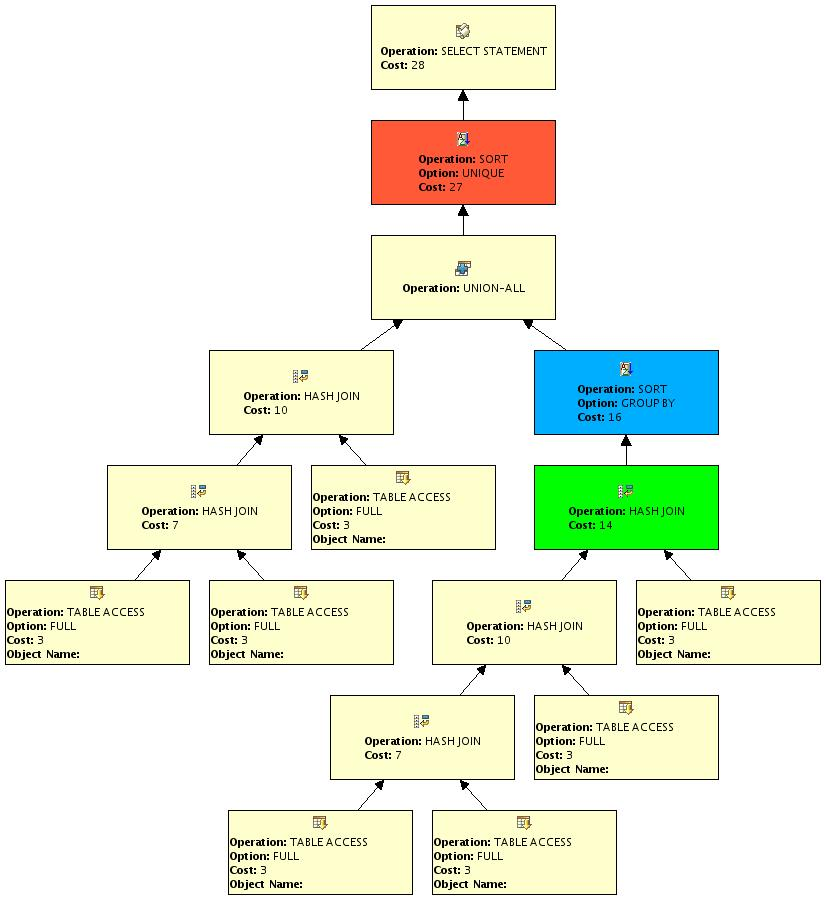
\includegraphics[width=0.7\textwidth]{Q3B}
\subsection*{Query C}
\begin{verbatim}
/* Starting innermost, this unions the (BID,StartYear,EndYear) of a
   member where there is a start year relating to that members time in
   a band with the (BID,StartYear,EarliestRelease) where the
   EarliestRelease is the earliest release for that band member in
   that band and where the start year is null.
*/
CREATE INDEX syear ON MEMBEROF(STARTYEAR)
go
CREATE INDEX bnames ON BAND(NAME)
go
CREATE INDEX RELEASEBIDS ON RELEASE(BID)
go
SELECT MEMBER.NAME as Guitarist_Name, Band.Name as Band_Name,
Mems.STARTYEAR as Start_Year, MEMS.ENDYEAR as END_YEAR
FROM MEMBER, BAND,
(
    (
        SELECT BAND.BID,MEMBEROF.MID, MEMBEROF.STARTYEAR As STARTYEAR,
        MEMBEROF.ENDYEAR as ENDYEAR
        FROM MEMBEROF,BAND,RELEASE
        WHERE MEMBEROF.STARTYEAR>0 AND MEMBEROF.INSTRUMENT='guitar'
        AND MEMBEROF.BID=BAND.BID AND BAND.BID=RELEASE.BID
    )
    UNION
    (
        SELECT BAND.BID, MEMBEROF.MID, MIN(RELEASE.YEAR) AS year,
        MEMBEROF.ENDYEAR
        FROM BAND, RELEASE, MEMBEROF
        WHERE BAND.BID=RELEASE.BID AND MEMBEROF.INSTRUMENT='guitar' 
        AND MEMBEROF.BID = BAND.BID AND (MEMBEROF.STARTYEAR IS NULL)
        GROUP BY MEMBEROF.MID, BAND.BID,MEMBEROF.ENDYEAR
    )
) MEMS
WHERE MEMS.MID=MEMBER.MID AND BAND.BID=MEMS.BID
ORDER BY MEMBER.NAME, MEMS.STARTYEAR
go
\end{verbatim}
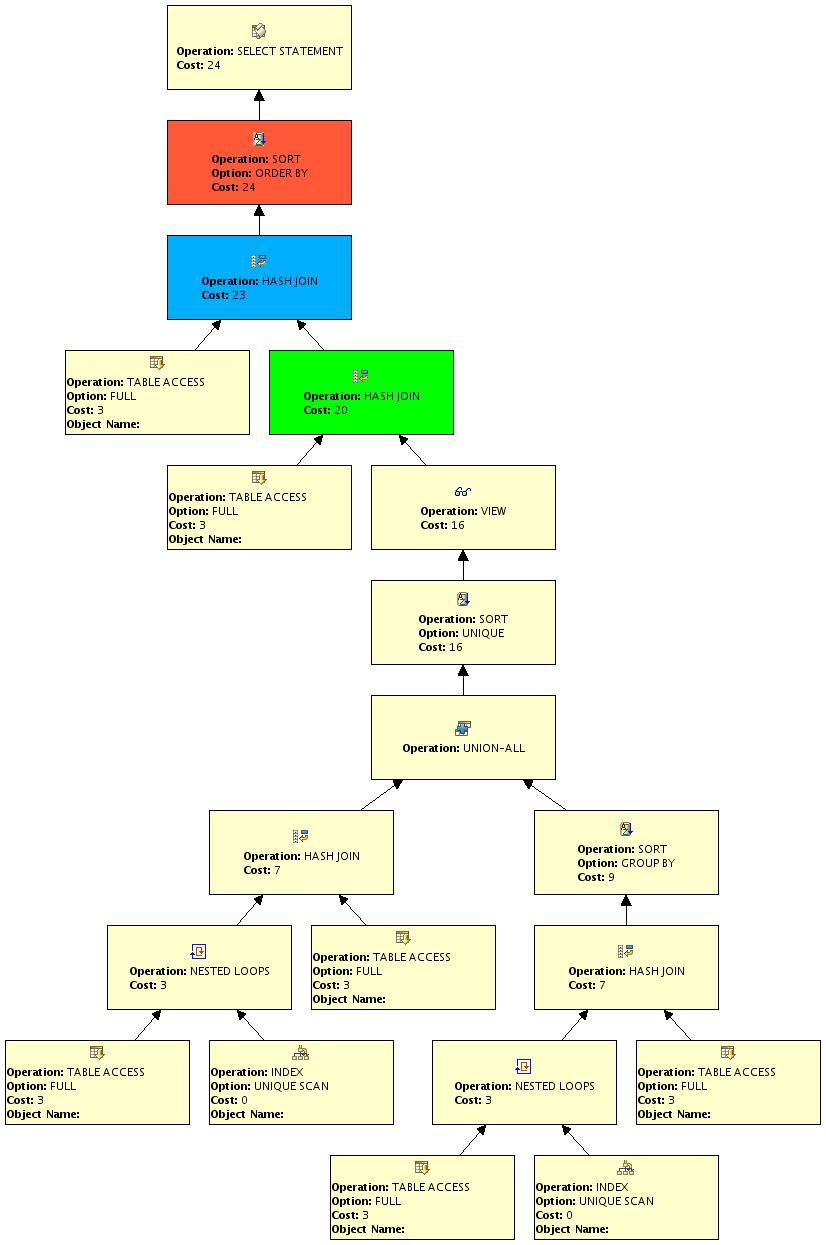
\includegraphics[width=0.7\textwidth]{Q3}
\subsection*{Output}
\begin{verbatim}
 GUITARIST_NAME         BAND_NAME           START_YEAR     END_YEAR    
 ---------------------  ------------------  -------------  ----------- 
 Adrian Smith           Iron Maiden         1981           1988        
 Adrian Smith           Bruce Dickinson     1997           1999        
 Adrian Smith           Iron Maiden         2000           (null)      
 Al Pitrelli            Savatage            1995           1998        
 Alex Skolnick          Savatage            1994           1994        
 Anders H. Hidle        Tristania           1997           (null)      
 Andre Olbrich          Blind Guardian      1990           (null)      
 Ben Jackson            Crimson Glory       1986           (null)      
 Chris Caffery          Savatage            1989           1989        
 Chris Caffery          Savatage            1995           (null)      
 Criss Oliva            Savatage            1985           1993        
 Dave Murray            Iron Maiden         1982           (null)      
 Frank Claussen         Theatre Of Tragedy  1998           (null)      
 Fredrik Johansson      Dark Tranquility    1999           1999        
 Geir Flikkeid          Theatre Of Tragedy  1996           1996        
 Janick Gers            Iron Maiden         1990           (null)      
 Jeff Loomis            Nevermore           1995           (null)      
 Jerry Fogle            Cirith Ungol        1984           1986        
 Jim Morris             Demons & Wizards    1999           1999        
 Jon Drenning           Crimson Glory       1986           (null)      
 Jon Schaffer           Iced Earth          1991           (null)      
 Jon Schaffer           Demons & Wizards    1999           (null)      
 Kai Hansen             Helloween           1985           1988        
 Kai Hansen             Gamma Ray           1989           (null)      
 Klas Bergwall          Candlemass          1986           1986        
 Larry Tarnowski        Iced Earth          1998           (null)      
 Lars Johansson         Candlemass          1987           1990        
 Lenny Rutledge         Sanctuary           1988           1990        
 Marcus Siepen          Blind Guardian      1990           (null)      
 Martin Henriksson      Dark Tranquility    2000           (null)      
 Mats Bjorkman          Candlemass          1986           1990        
 Michael Weikath        Helloween           1985           (null)      
 Mikael Akerfeldt       Opeth               1996           (null)      
 Mike Wead              Memento Mori        1993           1994        
 Morten Veland          Tristania           1997           (null)      
 Nikkey Argento         Memento Mori        1993           1994        
 Niklas Sundin          Dark Tranquility    1999           (null)      
 Pal Bjastad            Theatre Of Tragedy  1995           1995        
 Pat O'Brien            Nevermore           1996           1996        
 Peter Lindgren         Opeth               1996           (null)      
 Randy Shawver          Iced Earth          1991           1996        
 Roy Z                  Bruce Dickinson     1994           1999        
 Sean Blosl             Sanctuary           1988           1990        
 Stefan Kiefer          EverEve             1996           (null)      
 Thorsten Weibenberger  EverEve             1996           (null)      
 Tim Calvert            Nevermore           1999           1999        
 Tommy Lindal           Theatre Of Tragedy  1995           1996        
 Tommy Olsson           Theatre Of Tragedy  1998           (null)      
 Vorphalak              Samael              1995           (null)      

 49 record(s) selected
\end{verbatim}

%%%%%%%%%%%%%%%%%%%%%%%%%%%%%%%%%%%%%%%%%%%%%%%%%%%%%%%%%%%%%%%%%%%%%%%%%%
% Q4
%%%%%%%%%%%%%%%%%%%%%%%%%%%%%%%%%%%%%%%%%%%%%%%%%%%%%%%%%%%%%%%%%%%%%%%%%%
\section*{Query 4}
Query C is our optimized query. Query C is Query A optimized by
removing redundant code and changing the way we pass tuples through
the query. We considered using an index, but the benefits of the index
did not counterbalance the cost.
\subsection*{Query A}
\begin{verbatim}
/* The KPLAYERS Table is that of each keyboard player that has featured
   in a band.
   Band Left Outer Joins with this to give a table of all band names
   with either the keyboard players or nulls.
   Then the only check left is that the band name from band matches that
   of the keyboard player.
*/
SELECT BAND.NAME AS Band_Name, KPLAYERS.MNAME AS Keyboard_Player
FROM BAND LEFT OUTER JOIN 
(
    SELECT BAND.NAME AS BNAME, MEMBER.NAME AS MNAME 
    FROM BAND, MEMBER, MEMBEROF 
    WHERE MEMBEROF.INSTRUMENT = 'keyboards' 
    AND BAND.BID = MEMBEROF.BID 
    AND MEMBER.MID = MEMBEROF.MID 
    ) KPLAYERS
ON BAND.NAME = KPLAYERS.BNAME 
ORDER BY BAND.NAME
\end{verbatim}
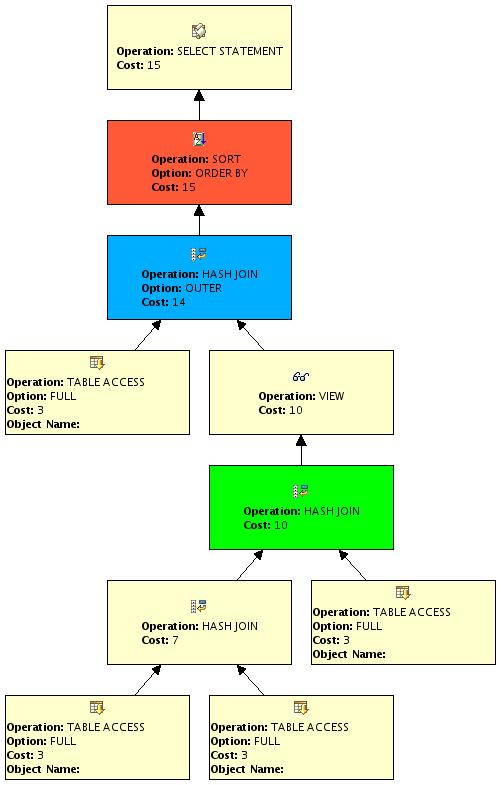
\includegraphics[width=0.7\textwidth]{Q4A}
\subsection*{Query B}
\begin{verbatim}
/* Finds keyboard players and nulls by creating a table with a left
   outer join between Band and any keyboard Players.
   Then filters this using MIDs and BIDs from MemberOf and Band,
   uses Distinct to remove duplicates that occur
*/
SELECT DISTINCT PLAYERS.BAND_NAME, PLAYERS.Keyboard_Player
FROM MEMBEROF, BAND, 
(
    SELECT BAND.NAME AS Band_Name, KEYS.NAME AS Keyboard_Player
    FROM BAND LEFT OUTER JOIN 
    (
        SELECT MEMBER.NAME,MEMBEROF.BID
        FROM MEMBEROF, MEMBER
        WHERE INSTRUMENT='keyboards' AND MEMBER.MID=MEMBEROF.MID
    )KEYS
ON BAND.BID=KEYS.BID
) PLAYERS
WHERE MEMBEROF.BID = BAND.BID
AND PLAYERS.Band_NAME = BAND.NAME
ORDER BY PLAYERS.BAND_NAME, PLAYERS.Keyboard_Player
\end{verbatim}
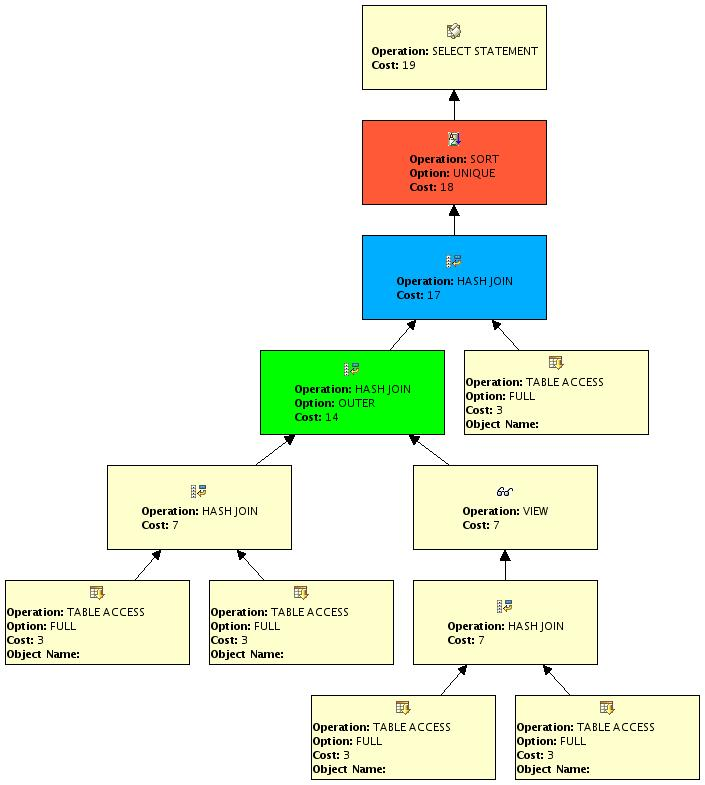
\includegraphics[width=0.7\textwidth]{Q4B}
\subsection*{Query C}
\begin{verbatim}
/* Selects all bands and the 'LEFT OUTER JOIN' allocates the band
   members which are keyboard players to their respective bands and
   inserts nulls in place for the other bands.
*/ 
SELECT BAND.NAME AS Band_Name, KEYS.NAME AS Keyboard_Player
FROM BAND
LEFT OUTER JOIN (
    SELECT MEMBER.NAME,MEMBEROF.BID
    FROM MEMBEROF, MEMBER
    WHERE INSTRUMENT='keyboards' AND MEMBER.MID=MEMBEROF.MID
    )KEYS
ON BAND.BID=KEYS.BID
ORDER BY BAND.NAME, KEYS.NAME
\end{verbatim}
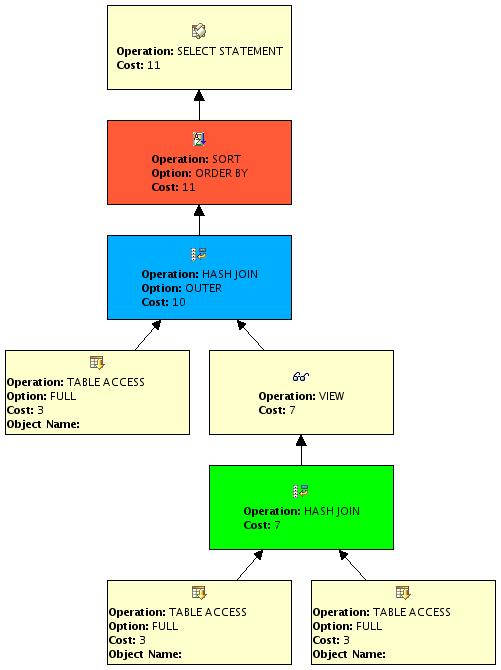
\includegraphics[width=0.7\textwidth]{Q4}
\subsection*{Output}
\begin{verbatim}
 BAND_NAME           KEYBOARD_PLAYER    
 ------------------  ------------------ 
 Blind Guardian      (null)             
 Bruce Dickinson     (null)             
 Candlemass          (null)             
 Cirith Ungol        (null)             
 Crimson Glory       (null)             
 Dark Tranquility    Martin Brandstrom  
 Demons & Wizards    (null)             
 EverEve             Michael Zeissl     
 Gamma Ray           (null)             
 Helloween           (null)             
 Iced Earth          (null)             
 Iron Maiden         (null)             
 Memento Mori        Miguel Robaina     
 Nevermore           (null)             
 Opeth               (null)             
 Samael              Rodolphe H.        
 Samael              Xy                 
 Sanctuary           (null)             
 Savatage            Jon Oliva          
 Theatre Of Tragedy  Lorentz Aspen      
 Tristania           Einar Moen         

 21 record(s) selected
\end{verbatim}

%%%%%%%%%%%%%%%%%%%%%%%%%%%%%%%%%%%%%%%%%%%%%%%%%%%%%%%%%%%%%%%%%%%%%%%%
% Q5
%%%%%%%%%%%%%%%%%%%%%%%%%%%%%%%%%%%%%%%%%%%%%%%%%%%%%%%%%%%%%%%%%%%%%%%%
\section*{Query 5}
\subsection*{Query A}
Query C is our optimized query. Both of our queries return the same
results for the given test data, but Query C will guarantee that there
is a singer on the top album returned. This was an intricacy
discovered too late for the change of one of our queries, so we are
aware that both queries may return different information depending on
the test data set.
The only optimization we could find for Query B (the one that
primarily guarantees a singer on the album) was to create an index on
the Members instruments. The cost of this is more than the saving of
the index, so this is only really valid if the query will be run more
than it is updated. However, and more interestingly, Query A will be
an optimization on Query B if there is a guarantee that every album
has a singer on the album.
\begin{verbatim}
/* ALLSONGS Shows every release by ID and its corresponding number of
   songs, which has been achieved here through a count. MAXSONGS uses
   a similar method to find the maximum number of songs that any album
   has. This means when they are inner joined, any releases that have
   the maximum number of songs are included, allowing for multiple
   albums to feature the most songs, for instance two could have 25
   and 25 could be the highest any has. What then happens is the
   singer is matched to a band through checks on foreign keys.
*/
SELECT BAND.NAME as Band_Name, MEMBER.NAME as Singer_Name,
RELEASE.TITLE AS Album_Name, THESONGS.SONG_NUMBER AS Song_Num
FROM RELEASE, MEMBER, MEMBEROF, BAND, 
(
    SELECT ALLSONGS.RID, ALLSONGS.NUM as Song_Number
    FROM 
    (
        SELECT RELEASE.RID as RID, count(SONG.TITLE)as NUM
        FROM RELEASE, SONG
        WHERE RELEASE.RID = SONG.RID
        GROUP BY RELEASE.RID
    ) ALLSONGS
    INNER JOIN
    (
        SELECT MAX(count(SONG.TITLE))as NUM
        FROM RELEASE, SONG
        WHERE RELEASE.RID = SONG.RID
        GROUP BY RELEASE.RID
    ) MAXSONGS 
    ON ALLSONGS.NUM = MAXSONGS.NUM
) THESONGS
WHERE RELEASE.RID = THESONGS.RID
AND RELEASE.BID = BAND.BID 
AND MEMBER.MID = MEMBEROF.MID
AND MEMBEROF.BID = BAND.BID
AND MEMBEROF.INSTRUMENT = 'vocals'
\end{verbatim}
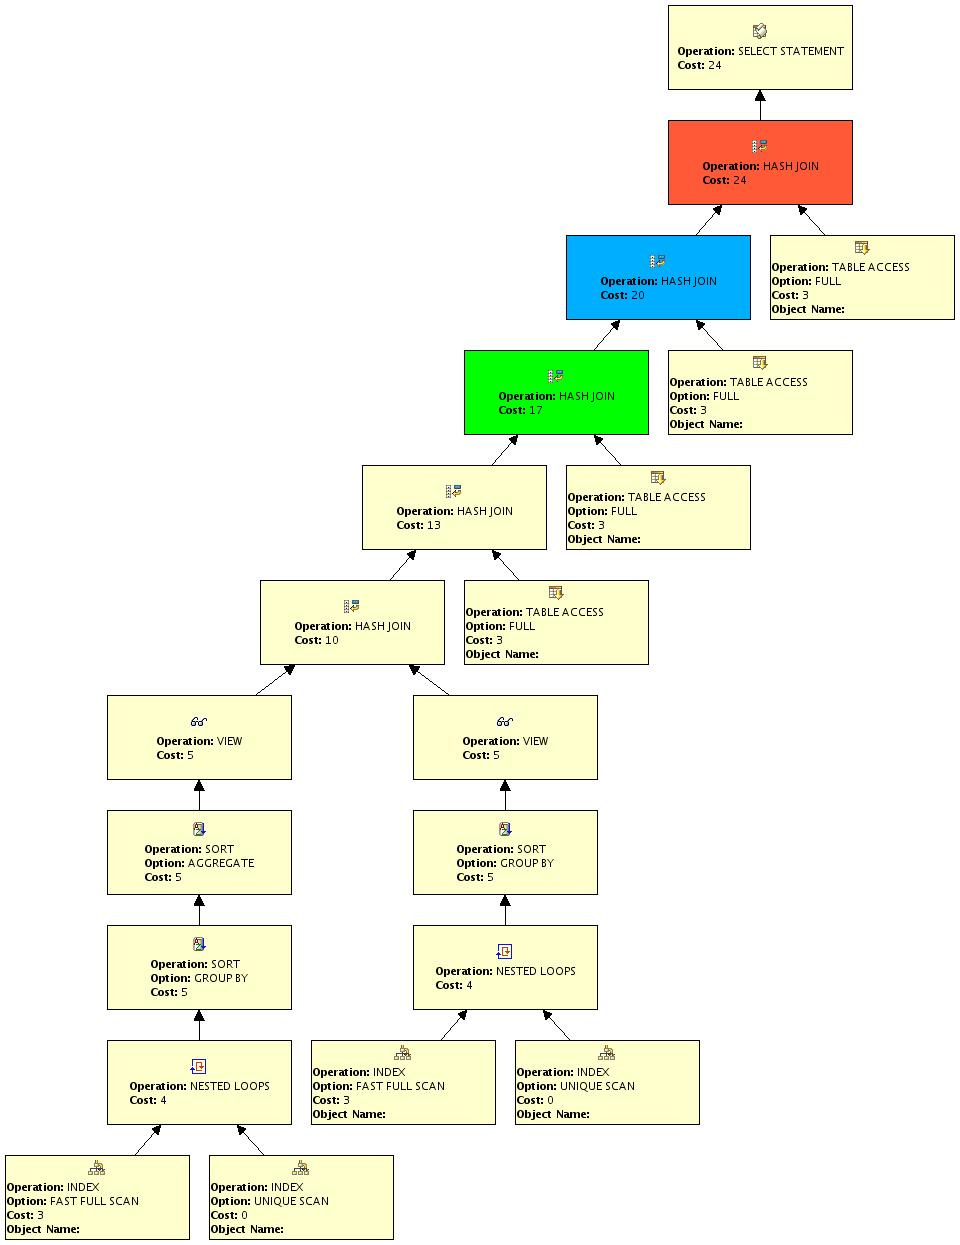
\includegraphics[width=0.7\textwidth]{Q5A}
\subsection*{Query B}
\begin{verbatim}
/* MostProlific picks the album with the largest number of songs that
   has a singer. This ensures that the album returned HAS a singer on
   the album. This is achieved by finding the number of tracks on the
   album with the most number of tracks that has a singer and then
   inner joining this with all the albums and the number of tracks on
   them. Then the singer is found for these albums.
*/
SELECT BAND.NAME AS Band_Name, MEMBER.NAME AS Singer_Name,
RELEASE.TITLE AS Album_Name, MostProlific.Total AS Song_Num
From BAND, RELEASE, MEMBEROF, MEMBER, 
(
    SELECT AlbumTracks.RID, AlbumTracks.Total
    FROM 
    (
        SELECT RELEASE.RID, COUNT(RELEASE.Title) AS total
        FROM RELEASE, SONG
        WHERE RELEASE.RID=SONG.RID 
        GROUP BY RELEASE.RID
        ORDER BY COUNT(RELEASE.Title) DESC
        ) AlbumTracks 
        INNER JOIN 
        (
        SELECT MAX(COUNT(RELEASE.Title)) AS total
        FROM RELEASE, SONG, MEMBEROF
        WHERE RELEASE.RID=SONG.RID AND RELEASE.BID=MEMBEROF.BID 
        AND 
        (   
             RELEASE.YEAR>=MEMBEROF.STARTYEAR 
             OR 
             MEMBEROF.STARTYEAR IS NULL
        )
        AND 
        (
             RELEASE.YEAR<=MEMBEROF.ENDYEAR 
             OR 
             MEMBEROF.ENDYEAR IS NULL
        ) 
        AND MEMBEROF.INSTRUMENT='vocals'
        GROUP BY RELEASE.RID
        ORDER BY COUNT(RELEASE.TITLE) DESC
    ) MostSongs
    ON AlbumTracks.total=MostSongs.total
) MostProlific
WHERE BAND.BID=Release.BID AND Release.RID=MostProlific.RID 
AND MEMBEROF.INSTRUMENT='vocals' AND MEMBEROF.MID=MEMBER.MID
AND (MEMBEROF.STARTYEAR <= Release.YEAR or MEMBEROF.STARTYEAR IS NULL)
AND (MEMBEROF.ENDYEAR >=RELEASE.YEAR OR MEMBEROF.ENDYEAR IS NULL) 
AND MEMBEROF.BID=BAND.BID
go
\end{verbatim}
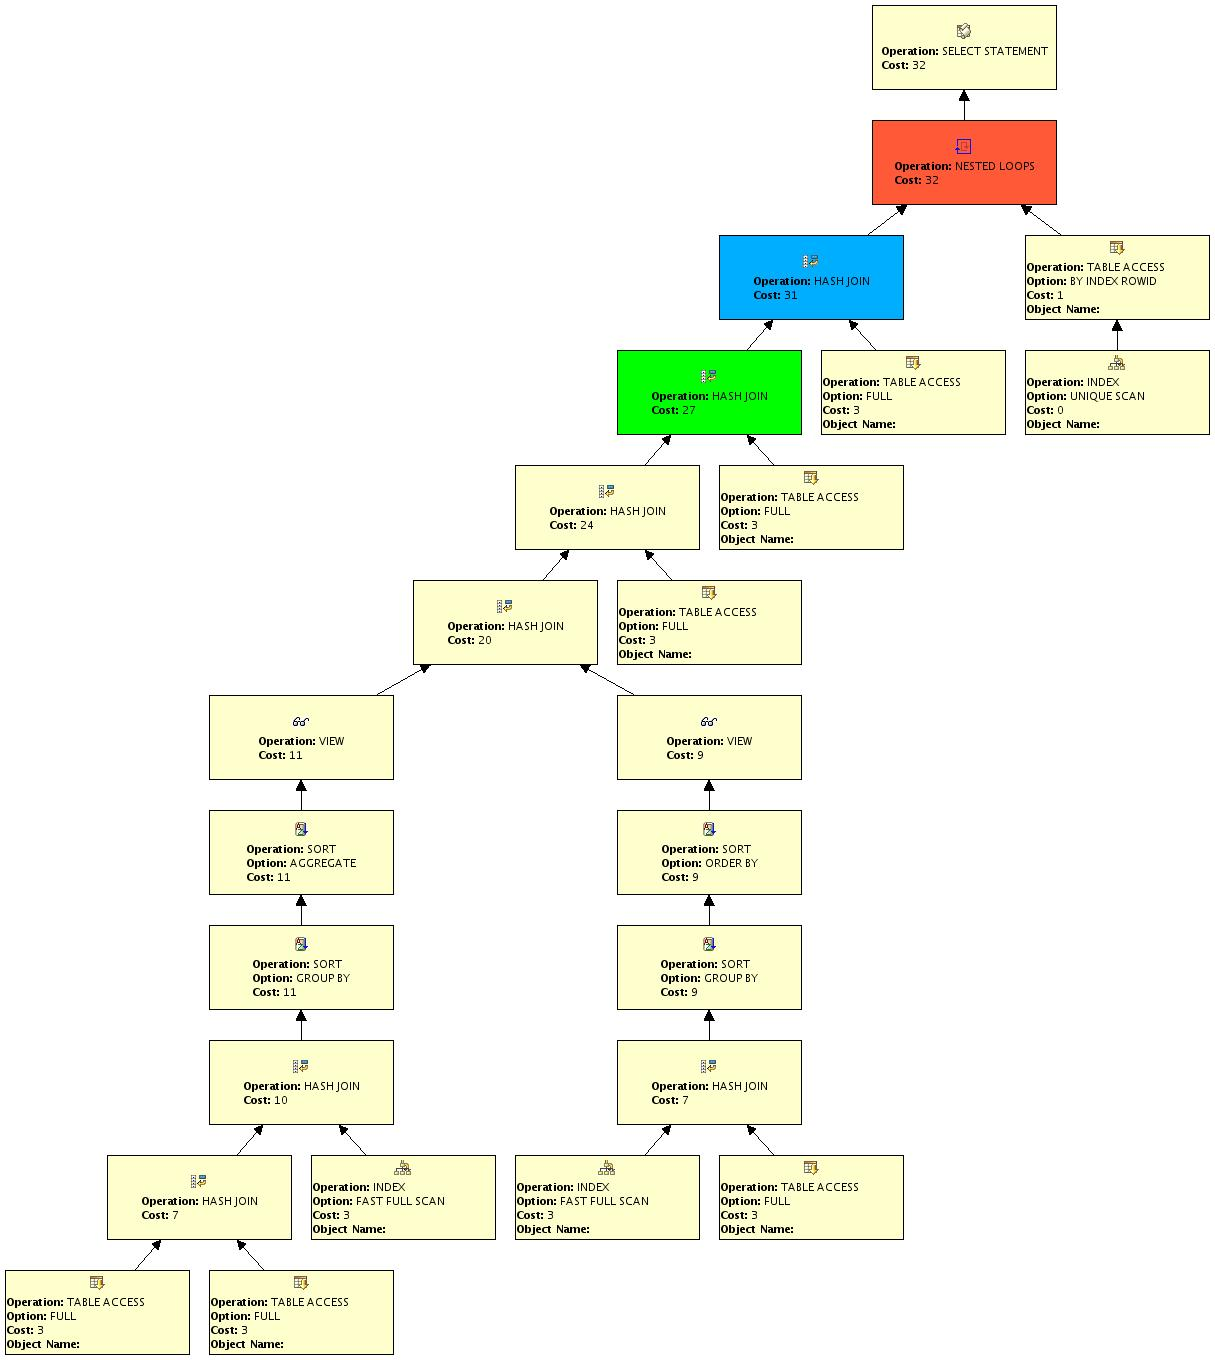
\includegraphics[width=0.7\textwidth]{Q5B}
\subsection*{Query C}
\begin{verbatim}
CREATE INDEX meminst on MemberOf(Instrument)
go
/* MostProlific picks the album with the largest number of songs that
   has a singer. This ensures that the album returned HAS a singer on
   the album. This is achieved by finding the number of tracks on the
   album with the most number of tracks that has a singer and then
   inner joining this with all the albums and the number of tracks on
   them. Then the singer is found for these albums.
*/
SELECT BAND.NAME AS Band_Name, MEMBER.NAME AS Singer_Name,
RELEASE.TITLE AS Album_Name, MostProlific.Total AS Song_Num
From BAND, RELEASE, MEMBEROF, MEMBER, 
(
    SELECT AlbumTracks.RID, AlbumTracks.Total
    FROM 
    (
        SELECT RELEASE.RID, COUNT(RELEASE.Title) AS total
        FROM RELEASE, SONG
        WHERE RELEASE.RID=SONG.RID 
        GROUP BY RELEASE.RID
        ORDER BY COUNT(RELEASE.Title) DESC
        ) AlbumTracks 
        INNER JOIN 
        (
        SELECT MAX(COUNT(RELEASE.Title)) AS total
        FROM RELEASE, SONG, MEMBEROF
        WHERE RELEASE.RID=SONG.RID AND RELEASE.BID=MEMBEROF.BID 
        AND 
        (   
             RELEASE.YEAR>=MEMBEROF.STARTYEAR 
             OR 
             MEMBEROF.STARTYEAR IS NULL
        )
        AND 
        (
             RELEASE.YEAR<=MEMBEROF.ENDYEAR 
             OR 
             MEMBEROF.ENDYEAR IS NULL
        ) 
        AND MEMBEROF.INSTRUMENT='vocals'
        GROUP BY RELEASE.RID
        ORDER BY COUNT(RELEASE.TITLE) DESC
    ) MostSongs
    ON AlbumTracks.total=MostSongs.total
) MostProlific
WHERE BAND.BID=Release.BID AND Release.RID=MostProlific.RID 
AND MEMBEROF.INSTRUMENT='vocals' AND MEMBEROF.MID=MEMBER.MID
AND (MEMBEROF.STARTYEAR <= Release.YEAR or MEMBEROF.STARTYEAR IS NULL)
AND (MEMBEROF.ENDYEAR >=RELEASE.YEAR OR MEMBEROF.ENDYEAR IS NULL) 
AND MEMBEROF.BID=BAND.BID
go
\end{verbatim}
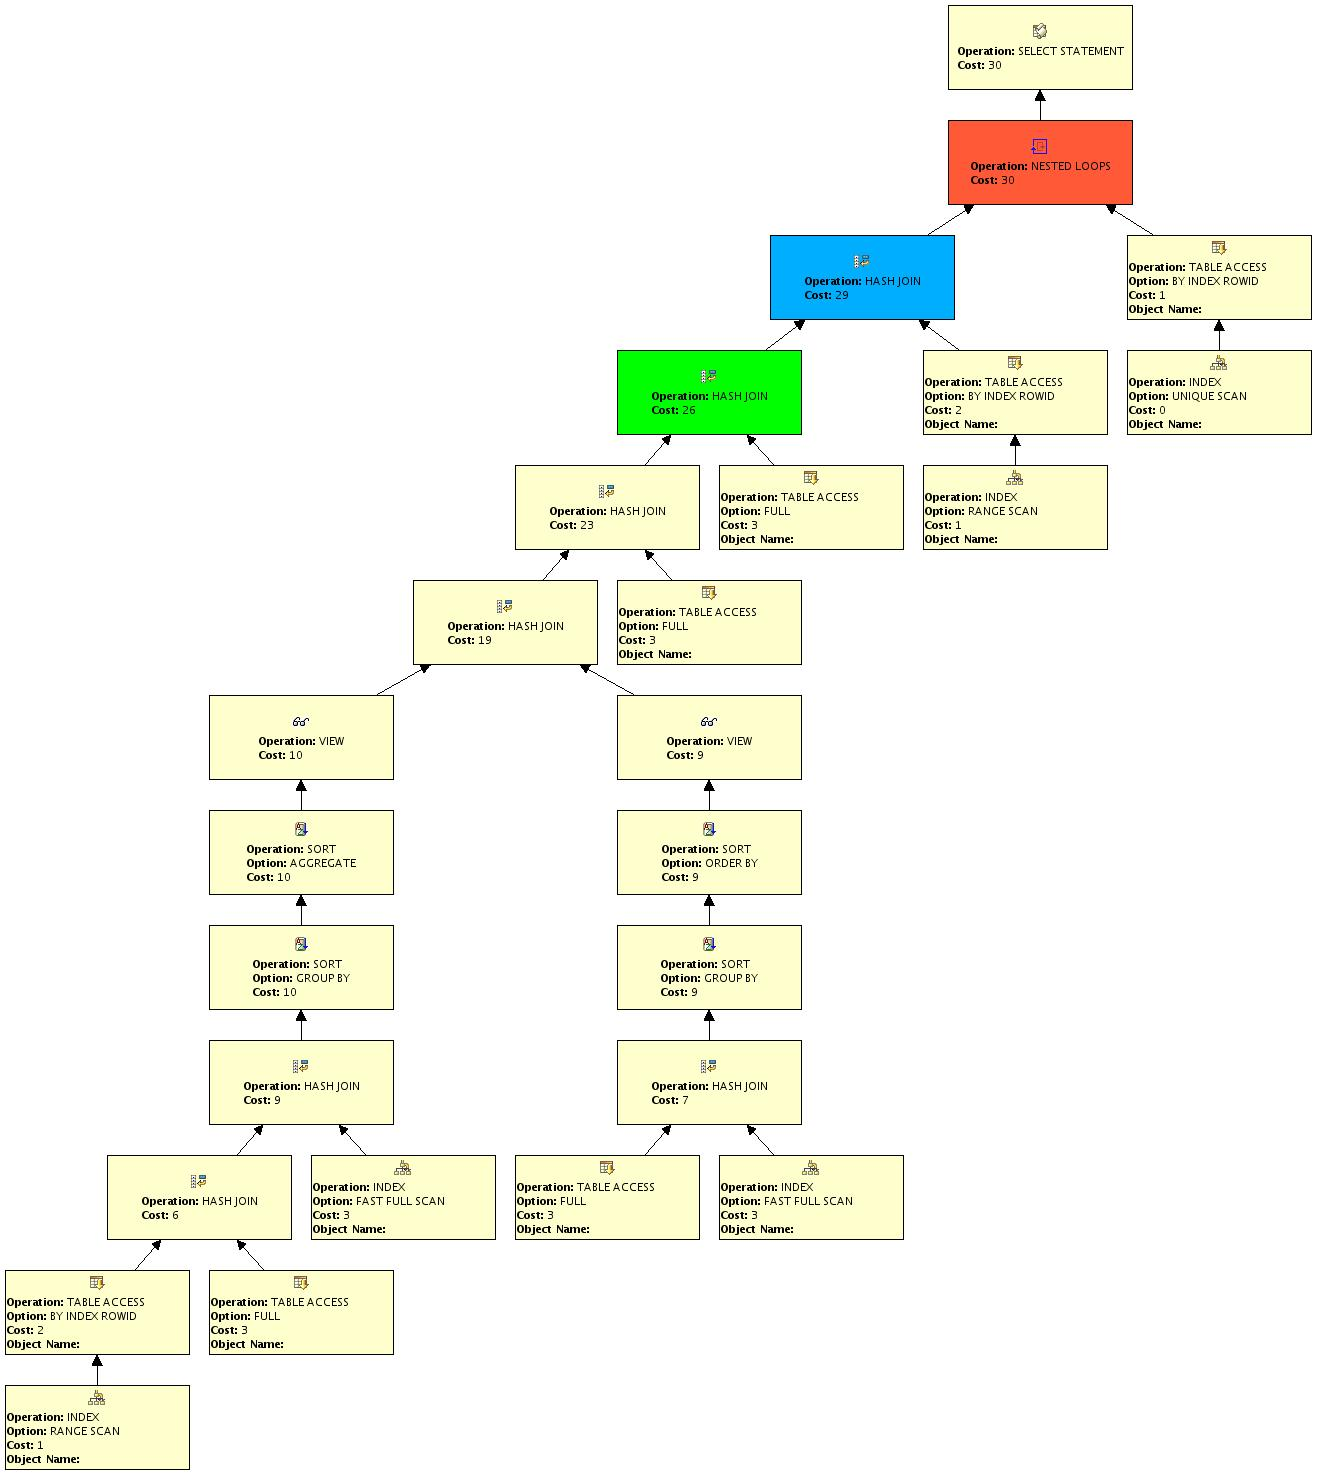
\includegraphics[width=0.7\textwidth]{Q5}
\subsection*{Output}
\begin{verbatim}
 BAND_NAME       SINGER_NAME     ALBUM_NAME                 SONG_NUM    
 --------------  --------------  -------------------------  ----------- 
 Blind Guardian  Hansi Kursch    Nightfall In Middle Earth  22          

 1 record(s) selected
\end{verbatim}
\end{document}